\documentclass[12pt]{amsart}
\setlength{\oddsidemargin}{0.3in} \setlength{\evensidemargin}{0.3in} \setlength{\textwidth}{6.2in}

\usepackage{amsmath}
\usepackage{amsthm}
\usepackage{amsfonts}
\usepackage{amssymb}
\usepackage{amscd}
\usepackage{stmaryrd}
\usepackage{hyperref}
\usepackage{enumerate}
\usepackage{graphicx}

% THEOREMS -------------------------------------------------------

\numberwithin{equation}{section}

\theoremstyle{plain}
\newtheorem{thm}[equation]{Theorem}
\newtheorem{lemma}[equation]{Lemma}
\newtheorem{cor}[equation]{Corollary}
\newtheorem{prop}[equation]{Proposition}

\theoremstyle{definition}
\newtheorem{definition}[equation]{Definition}
\newtheorem{example}[equation]{Example}
\newtheorem{question}[equation]{Question}
\newtheorem{remark}[equation]{Remark}


% MATH -----------------------------------------------------------
\newcommand{\PP}{\ensuremath \mathbb{P}}
\newcommand{\Q}{\ensuremath \mathbb{Q}}
\newcommand{\R}{\ensuremath \mathbb{R}}
\newcommand{\C}{\ensuremath \mathbb{C}}
\newcommand{\Z}{\ensuremath \mathbb{Z}}
\newcommand{\F}{\ensuremath \mathbb{F}}
\newcommand{\N}{\ensuremath \mathbb{N}}
\newcommand{\M}{\ensuremath \mathbb{M}}
\newcommand{\isom}{\ensuremath \cong}
\newcommand{\End}{\ensuremath{\mbox{\rm End}}}
\newcommand{\im}{\ensuremath{\mbox{\rm im}}}
\newcommand{\ann}{\ensuremath{\mbox{\rm ann}}}
\newcommand{\supp}{\ensuremath{\mbox{\rm supp}}}
\newcommand{\Nil}{\ensuremath{\mbox{\rm Nil}}}


\begin{document}

\section{The Simplex}

Let $\varepsilon\in [0,1)$ be a fixed constant.  Consider the symmetric half-cube
\[
R=\{(x,y,z)\in [0,2]^{3}\ :\ x+y+z\leq 3/2\}.
\]
We form the following seven subregions:
\begin{align*}
A_{xyz} & =\{(x,y,z)\in R\ :\ x+y\leq y+z\leq z+x\leq 1-\varepsilon\},\\
B_{xyz} & =\{(x,y,z)\in R\ :\ x+y\leq y+z\leq 1-\varepsilon\leq z+x\leq 1+\varepsilon\},\\
C_{xyz} & =\{(x,y,z)\in R\ :\ x+y\leq 1-\varepsilon \leq y+z \leq z+x\leq 1+\varepsilon\},\\
D_{xyz} & =\{(x,y,z)\in R\ :\ 1-\varepsilon \leq x+y\leq  y+z \leq z+x\leq 1+\varepsilon\},\\
E_{xyz} & =\{(x,y,z)\in R\ :\ x+y\leq y+z\leq 1-\varepsilon \leq  1+\varepsilon \leq z+x\},\\
F_{xyz} & =\{(x,y,z)\in R\ :\ x+y\leq 1-\varepsilon \leq y+z \leq  1+\varepsilon \leq z+x\},\\
G_{xyz} & =\{(x,y,z)\in R\ :\ x+y\leq 1-\varepsilon  \leq  1+\varepsilon \leq y+z \leq z+x\},\\
H_{xyz} & =\{(x,y,z)\in R\ :\ 1-\varepsilon \leq x+y\leq  y+z \leq 1+\varepsilon \leq z+x\}.
\end{align*}
Further, we define permutations of these sets by permuting the three variables $\{x,y,z\}$ both in the subscript and in the right half of the definition of the set.  These $6\times 8=48$ sets cover $R$.

It turns out that computationally we want to break up the region $F_{xyz}$ into three further subregions.  Namely
\begin{align*}
S_{xyz} & = \{(x,y,z)\in F_{xyz}\ :\ z\leq 1/2+\varepsilon\},\\
T_{xyz} & = \{(x,y,z)\in F_{xyz}\ :\ z\geq 1/2+\varepsilon;x\geq 1/2-\varepsilon \}, \\
U_{xyz} & = \{(x,y,z)\in F_{xyz}\ :\ x\leq 1/2-\varepsilon \}.
\end{align*}

Next, we define a function $F(x,y,z)$ (not to be confused with the $F_{xyz}$ region) which has polynomial support on those ten pieces, along with the obvious symmetries.  We assume further that $F|_{D_{xyz}}=0$.  So our function is really defined in terms of nine pieces of information.  Finally, we will be assuming that $\varepsilon\in [1/4,1/3]$, as one must use slightly different integrals in other ranges, and this seems to be the best range.

\section{The $I$-integral}

Given any function $F(x,y,z)$ defined on a 3-dimensional simplex $S$, we define the integral operator $I(S)=\int\int\int_{S}F(x,y,z)^2\ dx\ dy\ dz$.  To find $I:=I(R)$ it suffices to find the part of $I$ on each of the nine subregions we described in the previous section (we still ignore $D_{xyz}$), add them, and then multiply by 6.

We find on $A_{xyz}$ that
\[
I(A_{xyz})=\int_{x=0}^{1/2-\varepsilon/2}\int_{y=0}^{x}\int_{z=x}^{1-\varepsilon-x}F|_{A_{xyz}}^2\ dz\ dy\ dx.
\]
Next we compute
\[
I(B_{xyz})=\left(\int_{z=1/2-\varepsilon/2}^{1/2+\varepsilon/2}\int_{x=1-\varepsilon-z}^{z} +\int_{z=1/2+\varepsilon/2}^{1-\varepsilon}\int_{x=1-\varepsilon-z}^{1+\varepsilon-z}\right) \int_{y=0}^{1-\varepsilon-z}F|_{B_{xyz}}^2\ dy\ dx\ dz.
\]
Note that in this integral representation we require $\varepsilon<1/3$.  The computation on $C_{xyz}$ requires a bit more work, but we have
\begin{align*}
I(C_{xyz}) & = \left(\int_{y=0}^{1/2-3\varepsilon/2} \int_{x=y}^{y+2\varepsilon} + \int_{y=1/2-3\varepsilon/2}^{1/2-\varepsilon}\int_{x=y}^{1-\varepsilon-y} \right) \int_{z=1-\varepsilon-y}^{1+\varepsilon-x} \\ & + \int_{y=1/2-\varepsilon}^{1/2-\varepsilon/2}\int_{x=y}^{1-\varepsilon-y}\int_{z=1-\varepsilon-y}^{3/2-x-y} F|_{C_{xyz}}^2\ dz\ dx\ dy.
\end{align*}
Next, skipping over $D_{xyz}$, we find
\begin{align*}
I(E_{xyz}) & = \int_{z=1/2+\varepsilon/2}^{1-\varepsilon}\int_{x=1+\varepsilon-z}^{z}\int_{y=0}^{1-\varepsilon-z} F|_{E_{xyz}}^2\ dy\ dx\ dz.
\end{align*}
The region $F_{xyz}$ is somewhat complicated, but we broke it into three pieces.  We compute
\begin{align*}
I(S_{xyz}) & =  \left(\int_{y=0}^{1/2-3\varepsilon/2}\int_{z=1-\varepsilon-y}^{1/2+\varepsilon} +\int_{y=1/2-3\varepsilon/2}^{1/2-\varepsilon}\int_{z=y+2\varepsilon}^{1/2+\varepsilon} \right)\int_{x=1+\varepsilon-z}^{1-\varepsilon-y} F|_{S_{xyz}}\ dx\ dz\ dy
\end{align*}
while
\begin{align*}
I(T_{xyz}) &  = \left(\int_{z=1/2+\varepsilon}^{1/2+2\varepsilon}\int_{x=1+\varepsilon-z}^{3/2-z} + \int_{z=1/2+2\varepsilon}^{1+\varepsilon}\int_{x=1/2-\varepsilon}^{3/2-z}\right)\int_{y=0}^{3/2-x-z} F|_{T_{xyz}}^2\ dy\ dz\ dx
\end{align*}
and
\begin{align*}
I(U_{xyz}) & = \int_{x=0}^{1/2-\varepsilon}\int_{y=0}^{x}\int_{z=1+\varepsilon-x}^{1+\varepsilon-y} F|_{U_{xyz}}\ dz\ dy\ dx.
\end{align*}
The $G_{xyz}$ region contributes
\begin{align*}
I(G_{xyz}) & = \int_{x=0}^{1/2-\varepsilon}\int_{y=0}^{x}\int_{z=1+\varepsilon-y}^{3/2-x-y} F|_{G_{xyz}}^2\ dx\ dz\ dy.
\end{align*}
Our final region yields
\begin{align*}
I(H_{xyz}) & =\left(\int_{x=1/2+\varepsilon/2}^{1-\varepsilon}\int_{y=1-\varepsilon-x}^{3/2-2x} +\int_{x=1-\varepsilon}^{3/4}\int_{y=0}^{3/2-2x} \right) \int_{z=x}^{3/2-x-y}\\ & + \int_{x=1/2}^{1/2+\varepsilon/2}\int_{y=1-\varepsilon-x}^{1/2-\varepsilon}\int_{z=1+\varepsilon-x}^{3/2-x-y} F|_{H_{xyz}}^2\ dz\ dy\ dx.
\end{align*}


\section{The $J$-integral}

Similar to the previous section, we define the following integral operator: $J=J^{(3)}=\int\int_{(x,y,z)\in R\ :\ x+y\leq 1-\varepsilon}\left(\int_{z=0}^{\infty}F\ dz\right)^{2}\ dy\ dx$.  This integral can only be broken up so much, due to the presence of the squaring.  We will reduce to the case where $y\leq x$, so our integral passes through the regions $A_{xyz}$, $A_{yzx}$, $A_{zyx}$, $B_{xyz}$, $B_{zyx}$, $C_{xyz}$, $E_{xyz}$, $E_{zyx}$, $S_{xyz}$, $T_{xyz}$, $U_{xyz}$, and $G_{xyz}$.

Projecting all intersection lines of these regions to the $(x,y)$-plane, we have the diagram:
\begin{center}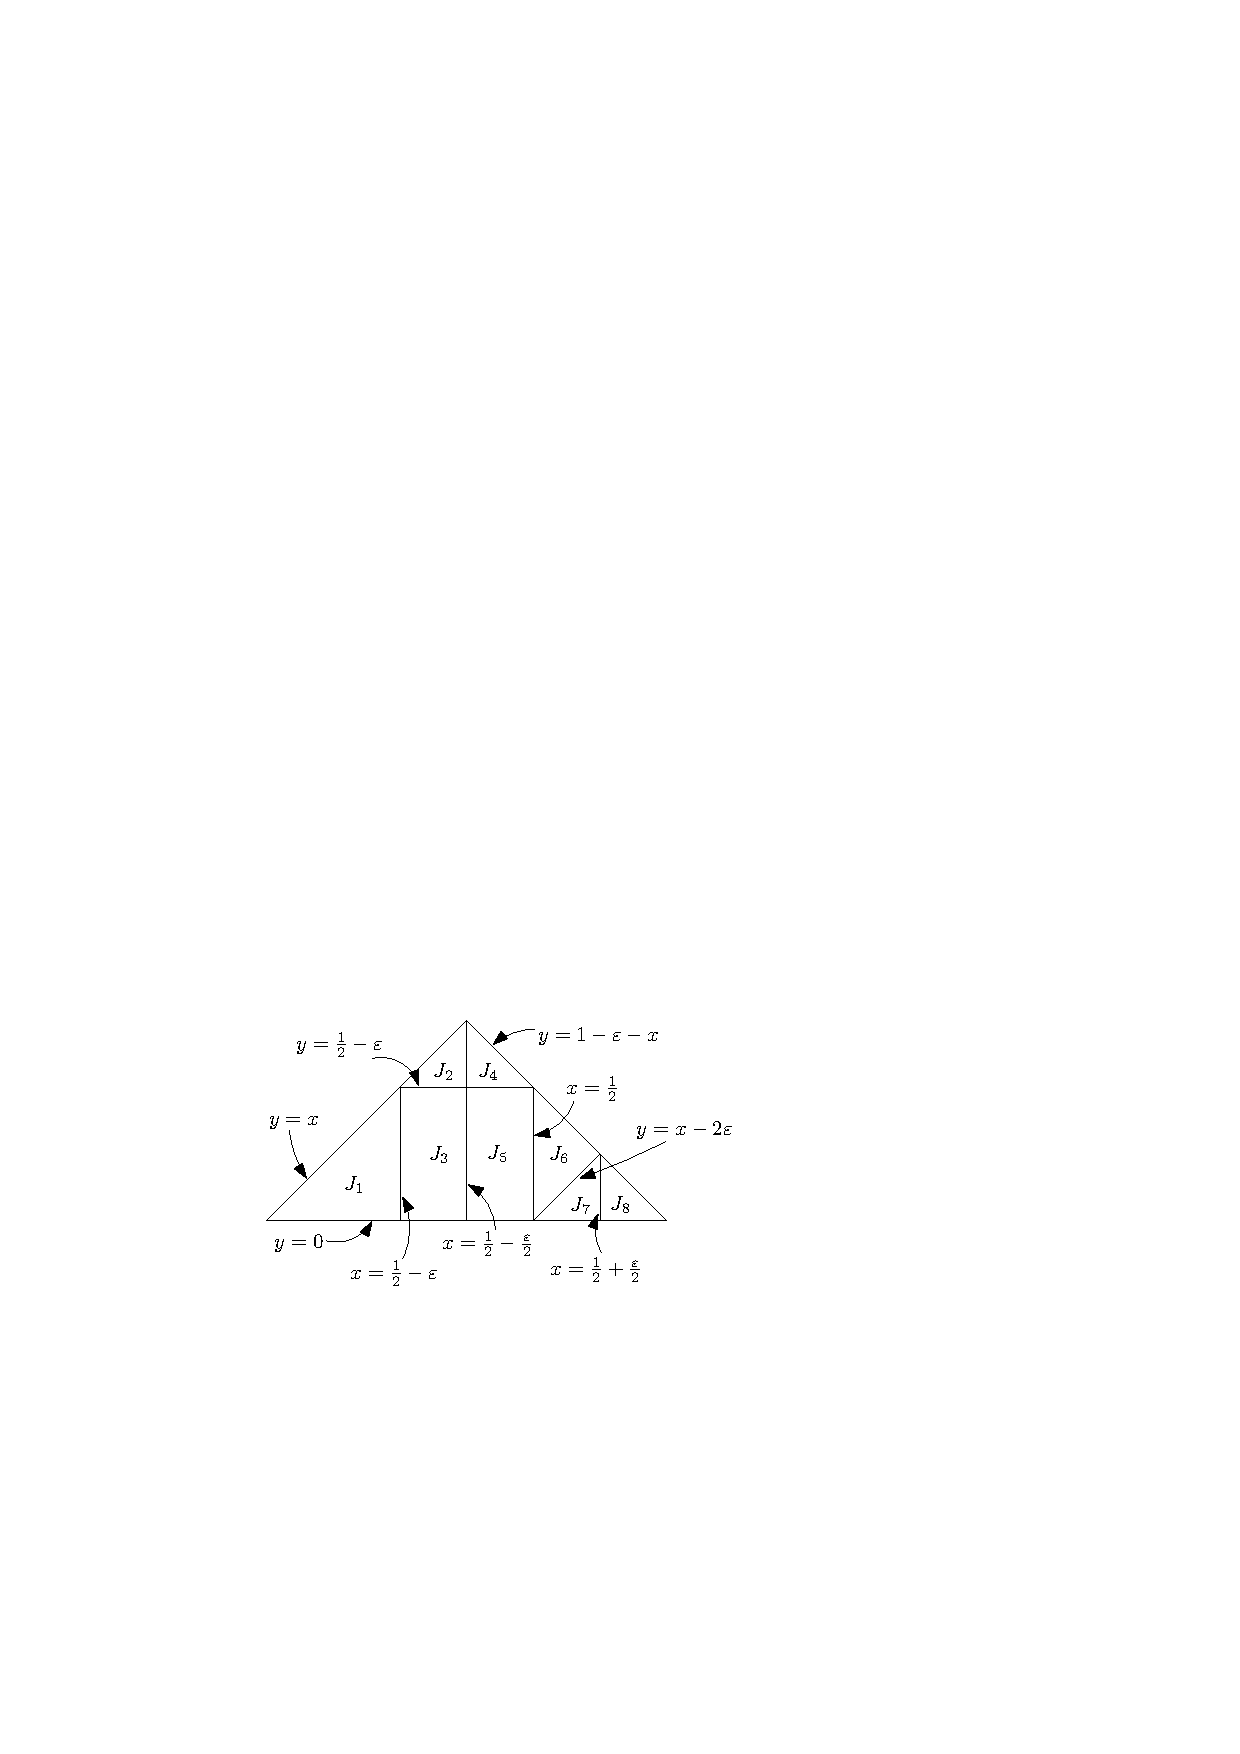
\includegraphics[scale=.5]{xyplot.pdf}\end{center}
The lines in this diagram, moving left to right (and then top to bottom) are $y=x$, $y=0$, $x=1/2-\varepsilon$, $y=1/2-\varepsilon$, $x=1/2-\varepsilon/2$, $x=1/2$, $y=x-2\varepsilon$, and $x=1/2+\varepsilon/2$.  This picture is only valid when $\varepsilon\in [1/4,1/3]$.  We label the pieces of the diagram moving from left to right and then top to bottom, and there are eight corresponding integrals $J1,J2,\ldots, J8$.

We have
\begin{align*}
J1 & =\int_{x=0}^{1/2-\varepsilon}\int_{y=0}^{x} \left(\int_{z=0}^{y}F|_{A_{yzx}}+\int_{z=y}^{x}F|_{A_{zyx}} +\int_{z=x}^{1-\varepsilon-x}F|_{A_{xyz}} +\int_{z=1-\varepsilon-x}^{1-\varepsilon-y}F|_{B_{xyz}}  \right. \\ & \left. +\int_{z=1-\varepsilon-y}^{1+\varepsilon-x}F|_{C_{xyz}} + \int_{z=1+\varepsilon-x}^{1+\varepsilon-y}F|_{U_{xyz}} + \int_{z=1+\varepsilon-y}^{3/2-x-y}F|_{G_{xyz}}\ dz \right)^{2}\ dy\ dx.
\end{align*}
Next comes
\begin{align*}
J2 & =\int_{x=1/2-\varepsilon}^{1/2-\varepsilon/2}\int_{y=1/2-\varepsilon}^{x} \left(\int_{z=0}^{y}F|_{A_{yzx}}+\int_{z=y}^{x}F|_{A_{zyx}}+\int_{z=x}^{1-\varepsilon-x}F|_{A_{xyz}} +\int_{z=1-\varepsilon-x}^{1-\varepsilon-y}F|_{B_{xyz}}\right. \\ & \left. +\int_{z=1-\varepsilon-y}^{3/2-x-y}F|_{C_{xyz}}\ dz \right)^{2}\ dy\ dx.
\end{align*}
Third is the piece
\begin{align*}
J3 & =\int_{x=1/2-\varepsilon}^{1/2-\varepsilon/2}\int_{y=0}^{1/2-\varepsilon} \left(\int_{z=0}^{y}F|_{A_{yzx}}+\int_{z=y}^{x}F|_{A_{zyx}} +\int_{z=x}^{1-\varepsilon-x}F|_{A_{xyz}} +\int_{z=1-\varepsilon-x}^{1-\varepsilon-y}F|_{B_{xyz}} \right. \\ & \left. + \int_{z=1-\varepsilon-y}^{1+\varepsilon-x}F|_{C_{xyz}} + \int_{z=1+\varepsilon-x}^{3/2-x-y}F|_{T_{xyz}}\ dz \right)^{2}\ dy\ dx.
\end{align*}

We now have dealt with all integrals involving $A_{xyz}$, and all remaining integrals pass through $B_{zyx}$.  Continuing, we have
\begin{align*}
J4 & =\int_{x=1/2-\varepsilon/2}^{1/2}\int_{y=1/2-\varepsilon}^{1-\varepsilon-x} \left(\int_{z=0}^{y}F|_{A_{yzx}}+\int_{z=y}^{1-\varepsilon-x}F|_{A_{zyx}} +\int_{z=1-\varepsilon-x}^{x}F|_{B_{zyx}} +\int_{z=x}^{1-\varepsilon-y}F|_{B_{xyz}}\right. \\ & \left. +\int_{z=1-\varepsilon-y}^{3/2-x-y}F|_{C_{xyz}}\ dz \right)^{2}\ dy\ dx.
\end{align*}
Another component is
\begin{align*}
J5 & = \int_{x=1/2-\varepsilon/2}^{1/2}\int_{y=0}^{1/2-\varepsilon} \left(\int_{z=0}^{y}F|_{A_{yzx}}+\int_{z=y}^{1-\varepsilon-x}F|_{A_{zyx}} \right. \\ & \left. +\int_{z=1-\varepsilon-x}^{x}F|_{B_{zyx}} +\int_{z=x}^{1-\varepsilon-y}F|_{B_{xyz}} +\int_{z=1-\varepsilon-y}^{1+\varepsilon-x}F|_{C_{xyz}} + \int_{z=1+\varepsilon-x}^{3/2-x-y}F|_{T_{xyz}}\ dz \right)^{2}\ dy\ dx.
\end{align*}

The most complicated piece is
\begin{align*}
J6 & =\left(\int_{x=1/2}^{2\varepsilon} \int_{y=0}^{1-\varepsilon-x} + \int_{x=2\varepsilon}^{1/2+\varepsilon/2}\int_{y=x-2\varepsilon}^{1-\varepsilon-x} \right) \left(\int_{z=0}^{y}F|_{A_{yzx}}+\int_{z=y}^{1-\varepsilon-x}F|_{A_{zyx}} +\int_{z=1-\varepsilon-x}^{x}F|_{B_{zyx}}  \right. \\ & \left. +\int_{z=x}^{1-\varepsilon-y}F|_{B_{xyz}} +\int_{z=1-\varepsilon-y}^{1+\varepsilon-x}F|_{C_{xyz}} + \int_{z=1+\varepsilon-x}^{1/2+\varepsilon}F|_{S_{xyz}}+ \int_{z=1/2+\varepsilon}^{3/2-x-y}F|_{T_{xyz}}\ dz \right)^{2}\ dy\ dx.
\end{align*}
We have now exhausted $C_{xyz}$.  The sixth piece is
\begin{align*}
J7 & = \int_{x=2\varepsilon}^{1/2+\varepsilon/2}\int_{y=0}^{x-2\varepsilon} \left(\int_{z=0}^{y}F|_{A_{yzx}}+\int_{z=y}^{1-\varepsilon-x}F|_{A_{zyx}} +\int_{z=1-\varepsilon-x}^{x}F|_{B_{zyx}} \right. \\ & \left. +\int_{z=x}^{1+\varepsilon-x}F|_{B_{xyz}} + \int_{z=1+\varepsilon-x}^{1-\varepsilon-y}F|_{E_{xyz}} + \int_{1-\varepsilon-y}^{1/2+\varepsilon}F|_{S_{xyz}}+ \int_{1/2+\varepsilon}^{3/2-x-y}F|_{T_{xyz}} \ dz \right)^{2}\ dy\ dx.
\end{align*}
Finally, we have
\begin{align*}
J8 & = \int_{x=1/2+\varepsilon/2}^{1-\varepsilon}\int_{y=0}^{1-\varepsilon-x} \left(\int_{z=0}^{y}F|_{A_{yzx}}+\int_{z=y}^{1-\varepsilon-x}F|_{A_{zyx}} +\int_{z=1-\varepsilon-x}^{1+\varepsilon-x}F|_{B_{zyx}} \right. \\ & \left. + \int_{z=1+\varepsilon-x}^{x}F|_{E_{zyx}} + \int_{z=x}^{1-\varepsilon-y}F|_{E_{xyz}} + \int_{1-\varepsilon-y}^{1/2+\varepsilon}F|_{S_{xyz}}+ \int_{1/2+\varepsilon}^{3/2-x-y}F|_{T_{xyz}}\ dz \right)^{2}\ dy\ dx.
\end{align*}
Adding up all of the previous integrals, and multiplying by 6, gives us the total contribution from all $J$-integrals, by symmetry.

\section{Marginals}

The marginal conditions are exactly that the following integrals must all be zero.
\begin{align*}
M1 & =\int_{z=0}^{3/2-x-y}F|_{G_{yzx}}\ dz\\
M2 & =\int_{z=0}^{y}F|_{G_{yzx}} +\int_{z=y}^{3/2-x-y}F|_{G_{zyx}}\ dz\\
M3 & =\int_{z=0}^{1+\varepsilon-x}F|_{U_{yzx}} + \int_{z=1+\varepsilon-x}^{y}F|_{G_{yzx}} +\int_{z=y}^{3/2-x-y}F|_{G_{zyx}}\ dz\\
M4 & =\int_{z=0}^{1+\varepsilon-x}F|_{U_{yzx}} + \int_{z=1+\varepsilon-x}^{3/2-x-y}F|_{G_{yzx}}\ dz\\
M5 & =\int_{z=0}^{3/2-x-y}F|_{T_{yzx}}\ dz\\
M6 & =\int_{z=0}^{1-\varepsilon-y}F|_{S_{yzx}} +\int_{z=1-\varepsilon-y}^{3/2-x-y}F|_{H_{yzx}} \ dz\\
M7 & =\int_{z=0}^{1-\varepsilon-x}F|_{E_{yzx}} + \int_{z=1-\varepsilon-x}^{1-\varepsilon-y}F|_{S_{yzx}} + \int_{z=1-\varepsilon-y}^{3/2-x-y}F|_{H_{yzx}}\ dz\\
M8 & =\int_{z=0}^{3/2-x-y}F|_{H_{yzx}}\ dz
\end{align*}

\section{The Computation}

All polynomials have monomials with only two variables appearing.  We take $F(x,y,z)$ to be a polynomial of degree 2 on each of $A_{xyz},B_{xyz},C_{xyz}$, and use degree 5 on the other six relevant components of $R$.  Optimizing the resulting quadratic form and taking $\varepsilon=1/4$, we get $M\geq 2.0009$.


\end{document} 